\paragraph{Requiredfunctionality}
Our initial plans for the animation were to make it depend on the actual user input in the exercise itself, particularly taking the sequence and the primers from the previous stages of the application. This was mainly to differentiate more from other similar PCR animations, like the ones demonstrated to us by the biology staff (\cite{anim1} , \cite{anim2}). Because of the high customisation requirements set by the task at hand and to provide maximum compatibility throughout the project we decded to develop the animation on Java utilising Java graphics package and Swing together, with the animation logic being developed from scratch. However, towards the end of the animation development it became apparent that the sequence required to be presented in the animation is just too large to be reasonably scaled with the individual nodes being visible. To extrapolate, the individual nodes were hard to make out as soon as the target PCR area reached about 150 nodes in length, which was not enough as the area could be well over that limit. Finally, as the clients were satisfied with a static animation, it was decided that we would just use the animation with a sample input that  was adequately sized. It was also suggested by the biology staff that the individual nodes' color coding doesn't need to be explained in the animation as it was clear enough that the different colors represent different node types. Otherwise the aforementioned shift in the overarching animation design didn't affect it in any way. The final animation sreenshots and explanation of its individual parts are provided below.

\paragraph{Implementation}
The whole animation is controlled with a large set of conditional statements by a swing timer that constantly recalculates the time passed from the start of the animation, pausing if it reaches the end of a stage until a button press changes the stange and therefore sets the time passed to a particular value. The models used in the animation were developed in the Inkscape vector graphics editor and are the different type of the individual nodes models, the taq polymerase model and three models for three different states of the thermometer. The individual nodes are then drawn to make a sequence at a particular location.

\paragraph{Functionalityexplained}
The animation is split into 7 stages, with each one having a text about the animation at the bottom. The bottom line in small font size indicates the current stage of the animation, with the complicated stages having a short explanation of the stages in brakets, and the state of that stage, which can be "in progress" or "finished". The thermometer in the bottom right part of the sreen is shifting between three possible states, according to the three temperature levels required by PCR: 55°C, the average melting temperature of primers; 72°C, the temperature at which the Taq DNA polymerase synthesizes complementary strands; 95°C, the temperature of denaturation (DNA individual strand separation). The four buttons above the text are: "Close", to close the application completely; "Restart", to go to the start of the exercise; "Previous" and "Next" to navigate between the animation stages. The animation won't proceed until the "Next" button is pressed, something which was suggested by the biology staff, as they pointed out that the user might not be able to read the text in the time provided. Finally, the PCR animation itself is in the top part of the screen.

\paragraph{AnimationScreens}

In the stages 0 and 1, the user is explained what PCR is and what ingredients it requires as the temperature goes up to 72°C.

\begin{figure}[h]
  \begin{center}
	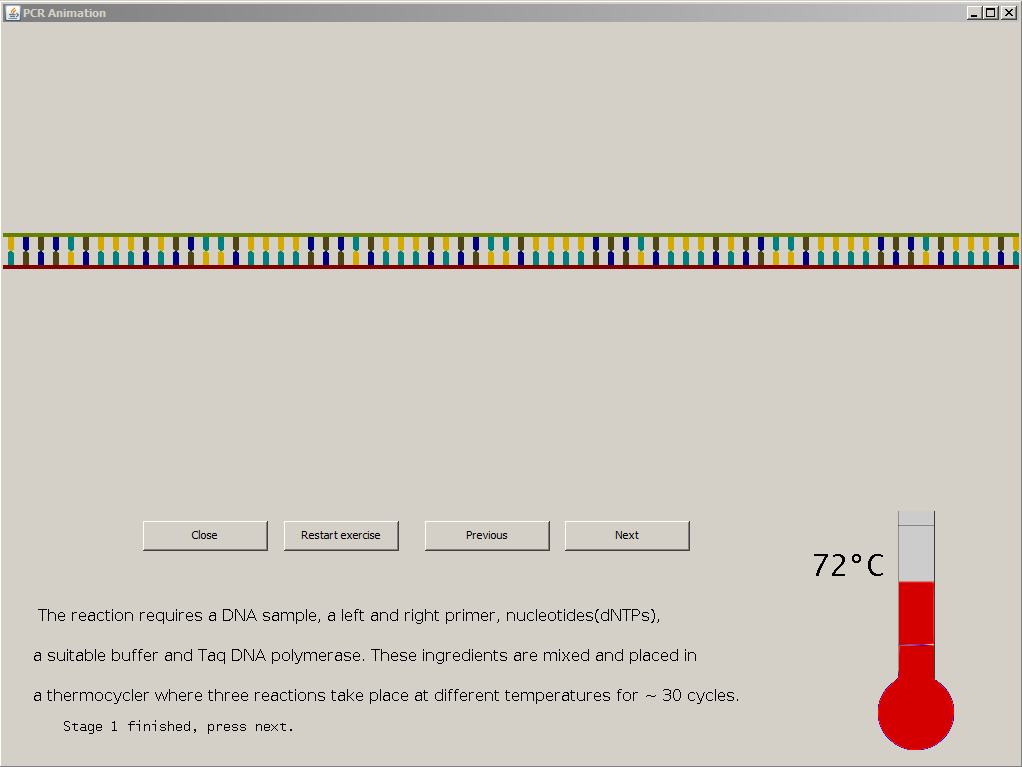
\includegraphics[width=0.6\textwidth]{./images/AnimImpl/Stage1.png}
    \caption{
      \label{fig:AnimImpl:stage1}
      Animation, stage1
    }
  \end{center}
\end{figure}


In stage 2, Melting and Annealing, the strands are separated and the primers bind to them, with the temperature level varying accordingly.

\begin{figure}[h]
  \begin{center}
	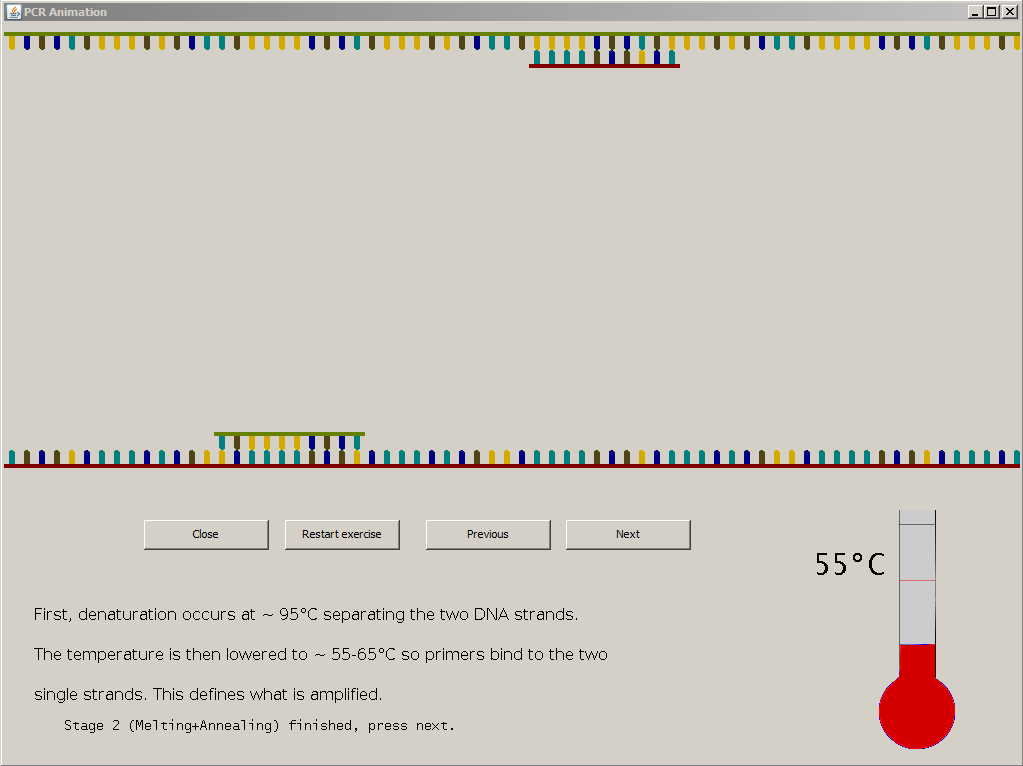
\includegraphics[width=0.6\textwidth]{./images/AnimImpl/Stage2.png}
    \caption{
      \label{fig:AnimImpl:stage2}
      Animation, stage2
    }
  \end{center}
\end{figure}

In stage 3, Adding nucleotides, the taq polymerase creates a complementary copy of each strand, with the temperature once again raised to 72°C.

\begin{figure}[h]
  \begin{center}
	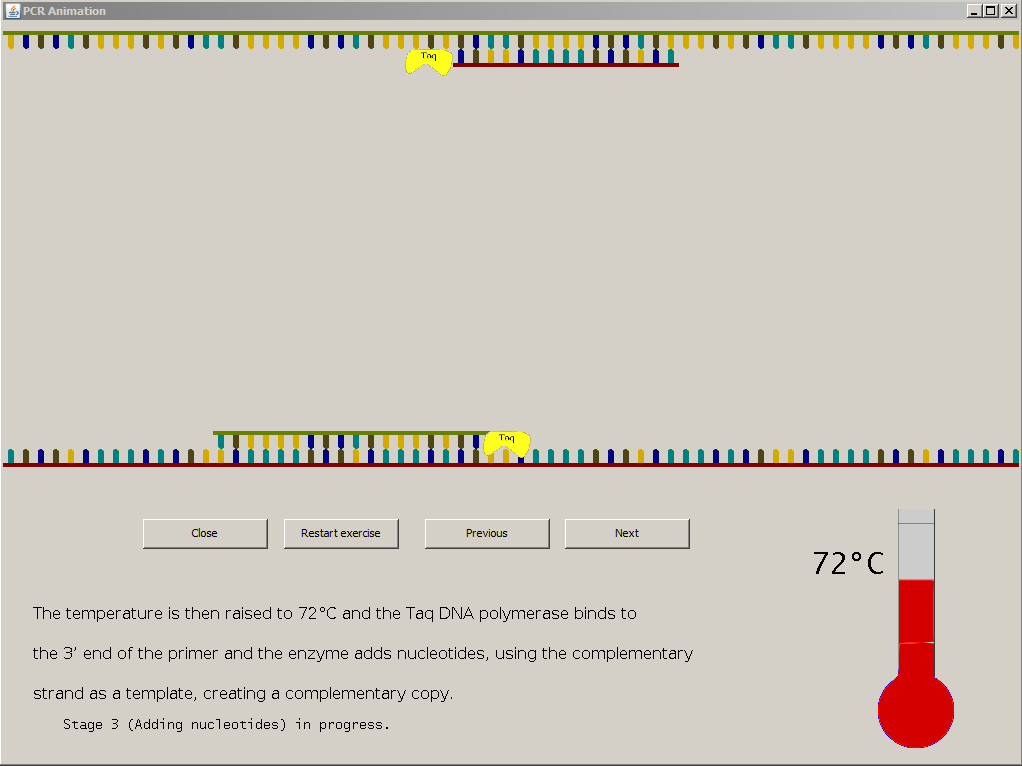
\includegraphics[width=0.6\textwidth]{./images/AnimImpl/Stage3.png}
    \caption{
      \label{fig:AnimImpl:stage3}
      Animation, stage3
    }
  \end{center}
\end{figure}

In stages 4 and 5 another cycle of PCR is shown and the required sequence is generated for the first time.

\begin{figure}[h]
  \begin{center}
	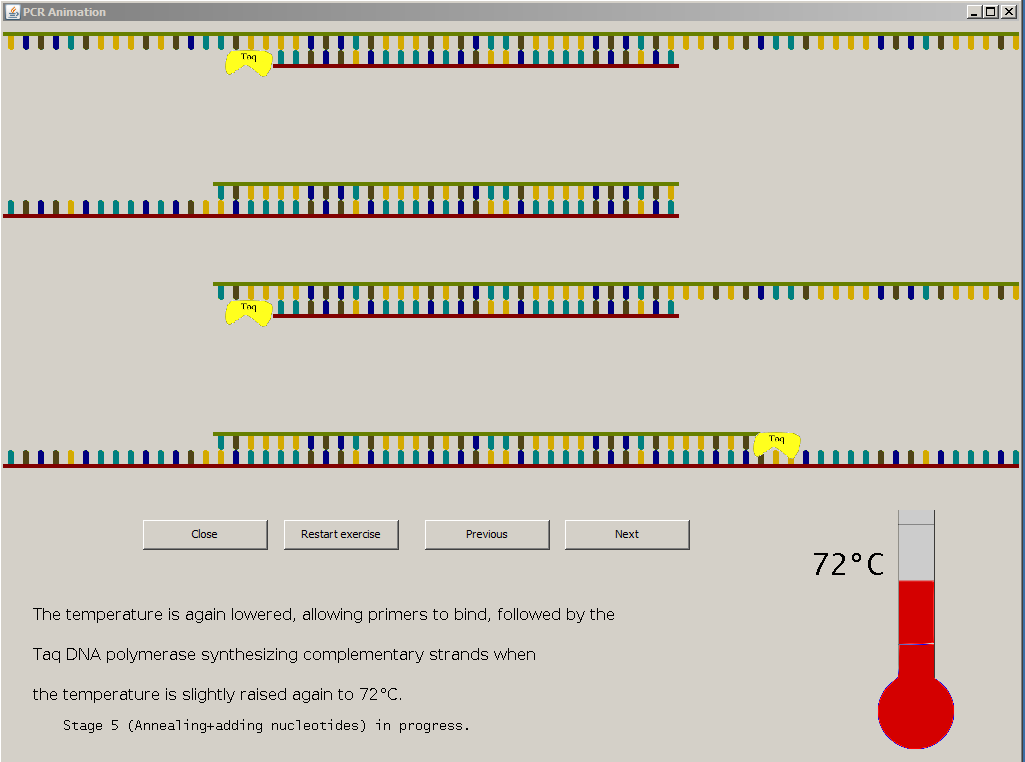
\includegraphics[width=0.6\textwidth]{./images/AnimImpl/Stage5.png}
    \caption{
      \label{fig:AnimImpl:stage5}
      Animation, stage5
    }
  \end{center}
\end{figure}

Finally, the last two stages explain how many copies of the target sequence is produced in subsequent cycles and the user is explained that he completed the exercise and thanked for participation.

\begin{figure}[h]
  \begin{center}
	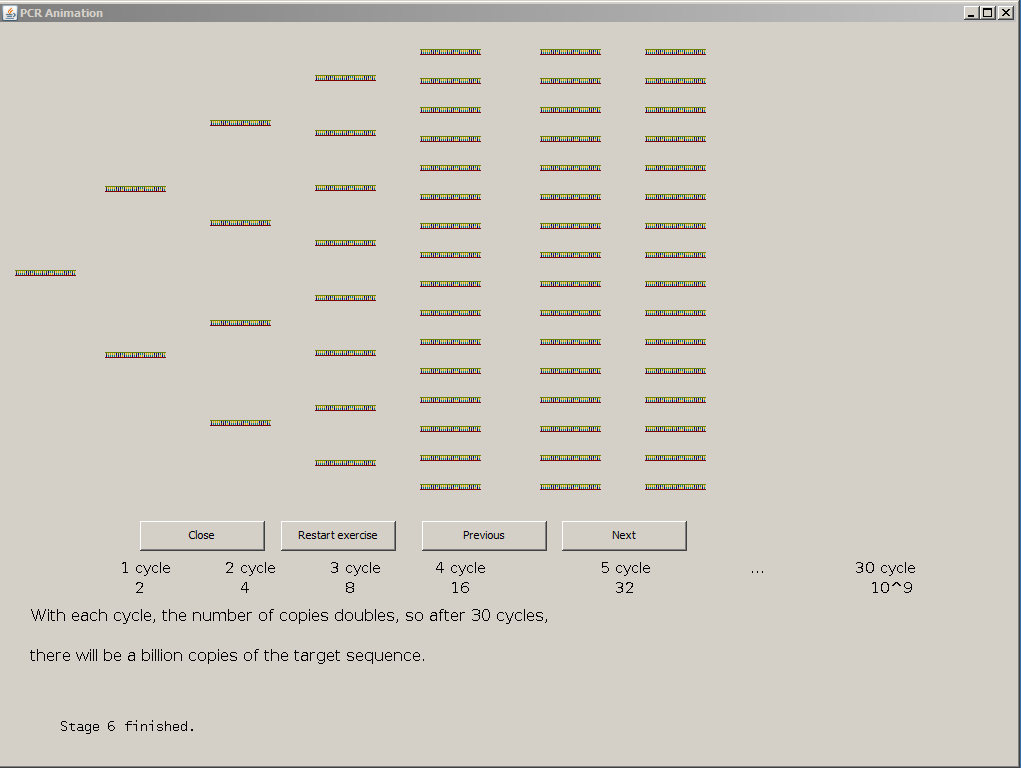
\includegraphics[width=0.6\textwidth]{./images/AnimImpl/Stage6.png}
    \caption{
      \label{fig:AnimImpl:stage6}
      Animation, stage6
    }
  \end{center}
\end{figure}
